\documentclass{article}
\usepackage[utf8]{inputenc}

\title{MLT Homework 4}
\author{Ana Borovac \\ Jonas Haslbeck \\ Bas Haver}

\usepackage{natbib}
\usepackage{graphicx}
\usepackage{subcaption}

\usepackage{amsmath}
\usepackage{amsfonts}
\usepackage{amssymb}
\usepackage{bbm}
\usepackage{mathtools}

\usepackage{url}

\DeclarePairedDelimiter\ceil{\lceil}{\rceil}
\DeclarePairedDelimiter\floor{\lfloor}{\rfloor}

\newcounter{counterquestion}
\newenvironment{question}[1]
{
\stepcounter{counterquestion}
\section*{Question \thecounterquestion}
\emph{#1} 
} 
{
}

\newcounter{countersubquestion}[counterquestion]
\newenvironment{subquestion}[1]
{
\stepcounter{countersubquestion}
\subsection*{Subquestion \thecounterquestion .\thecountersubquestion}
\emph{#1} 
} 
{
}

\newenvironment{solution}
{
\subsubsection*{Solution}
} 
{
}


\begin{document}

\maketitle

% 1st question
\begin{question}{We have shown that for a finite hypothesis class $\mathcal{H}$, $\text{VCdim}(\mathcal{H}) \leq \floor*{\log(|\mathcal{H}|)}$. However, this is just an upper bound. The VC-dimension of a class can be much lower than that.}
\begin{subquestion}{Find an example of a class $\mathcal{H}$ of functions over the real interval $\mathcal{X} = [0, 1]$ such that $\mathcal{H}$ is infinite while $\text{VCdim}(\mathcal{H}) = 1$.}
\begin{solution}
Let's define hypothesis class as:
\[
\mathcal{H} = \{h_{a}:\ a \in [0, 1]\}
\]
\[
h_{a}(x) = 
\begin{cases}
1; & x \geq a \\
0; & x < a \\
\end{cases} 
\]
%
From definition we know $|\mathcal{H}| = \infty$. Now we need to prove that $\text{VCdim}(\mathcal{H}) = 1$.

\begin{figure}[h!]
    \centering
    \begin{subfigure}[t]{0.4\textwidth}
        \centering
        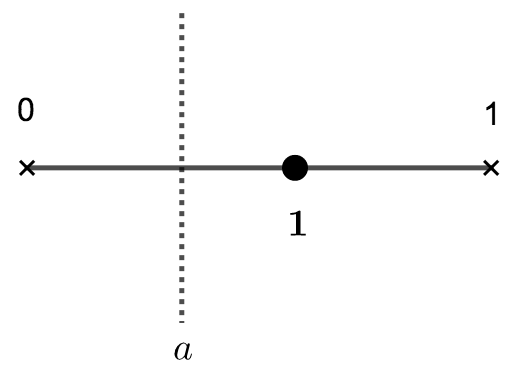
\includegraphics[width=0.9\textwidth]{Question11.png}
        \caption{If point is labeled “1”.}
    \end{subfigure}
    \begin{subfigure}[t]{0.4\textwidth}
        \centering
        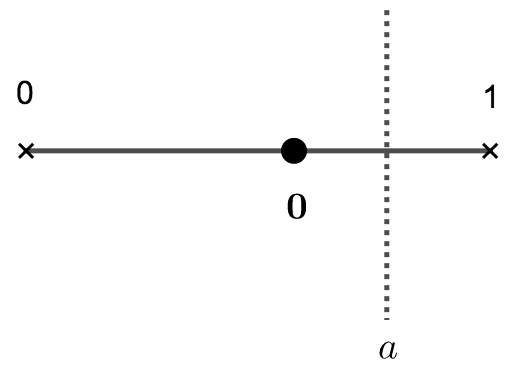
\includegraphics[width=0.9\textwidth]{Question12.png}
        \caption{If point is labeled “0”.}
    \end{subfigure}
    \caption{Proof that $\text{VCdim}(\mathcal{H}) \geq 1$.}
    \label{fig: question111}
\end{figure}

\begin{itemize}
\item $\text{VCdim}(\mathcal{H}) \geq 1$: The proof we can see from the figure \ref{fig: question111}.
\item $\text{VCdim}(\mathcal{H}) \leq 1$: From the figure \ref{fig: question112} it is seen that hypothesis class $\mathcal{H}$ does not shatter a set of two points (no matter how we position them).
\end{itemize}

\begin{figure}[h!]
\centering
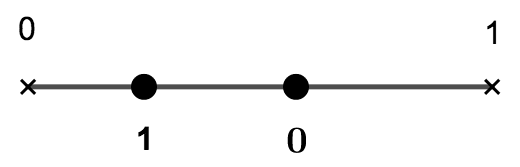
\includegraphics[width=0.5\textwidth]{Question13.png}
\caption{The problem we have when trying to shatter a set of two points.}
\label{fig: question112}
\end{figure}
\end{solution}
\end{subquestion}

\begin{subquestion}{Give an example of a finite hypothesis class $\mathcal{H}$ over domain $\mathcal{X} = [0, 1]$, where $\text{VCdim}(\mathcal{H}) = \floor*{\log_2(|\mathcal{H}|)}$}
\begin{solution}
Let's define hypothesis class:
\[
\mathcal{H} = \{h_0, h_1\}
\]
where $h_0(x) = 0$ ($\forall x$) and $h_1(x) = 1$ ($\forall x$). We would like to prove that $\text{VCdim}(\mathcal{H}) =  \floor*{\log_2(|\mathcal{H}|)} =  \floor*{\log_2(2)} = 1$.
\begin{itemize}
\item $\text{VCdim}(\mathcal{H}) \geq 1$: If we want to label a $x \in [0, 1]$ as 1, we pick $h_1$ as hypothesis, otherwise we pick $h_0$. So, $\text{VCdim}(\mathcal{H}) \geq 1$.
\item $\text{VCdim}(\mathcal{H}) \leq 1$: Let say that we have a set of two points. If we want to label one of the point with 1 and the other with 0, there does not exist a hypothesis in hypothesis class which can label two points differently. 
\end{itemize}
We can conclude that $\text{VCdim}(\mathcal{H}) = 1$.
\end{solution}
\end{subquestion}
\end{question}


% 2nd question
\begin{question}{6.8}
\begin{solution}

\end{solution}
\end{question}


% 3rd question
\begin{question}{Let $\mathcal{H}$ be the class of signed intervals, that is, $\mathcal{H} = \{h_{a, b, s} : a \leq b, s \in \{-1, 1\}\}$ where
\[
h_{a, b, s}(x) =
\begin{cases}
s & \text{if}\ x \in [a, b] \\
-s & \text{if}\ x \notin [a, b] 
\end{cases}
\]
Calculate $\text{VCdim}(\mathcal{H})$.}
\begin{solution}
Claim: $\text{VCdim}(\mathcal{H}) = 3$.

\begin{itemize}
\item $\text{VCdim}(\mathcal{H}) \geq 3$: On figure \ref{fig: question31} it is seen that set of three points can be shattered. Furthermore $\text{VCdim}(\mathcal{H}) \geq 3$.

\begin{figure}[h!]
    \centering
    \begin{subfigure}[t]{0.4\textwidth}
        \centering
        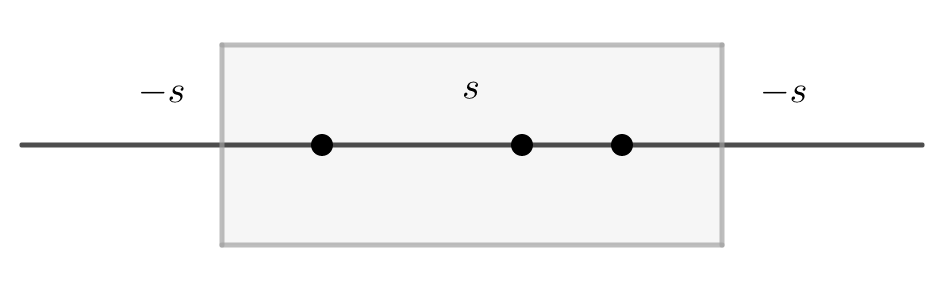
\includegraphics[width=0.9\textwidth]{Question31.png}
        \caption{}
    \end{subfigure}
    \begin{subfigure}[t]{0.4\textwidth}
        \centering
        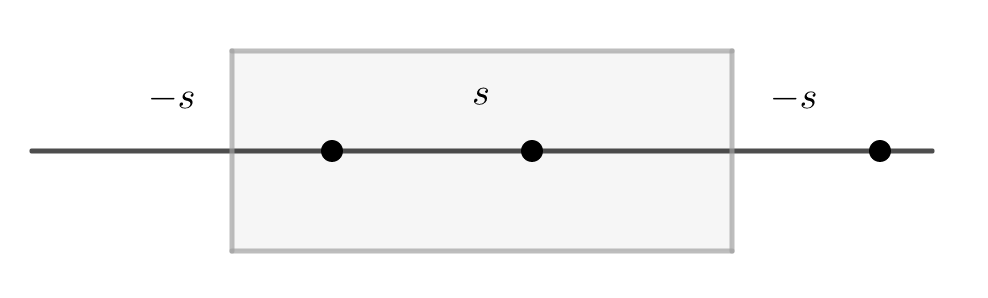
\includegraphics[width=0.9\textwidth]{Question32.png}
        \caption{}
    \end{subfigure}
     \begin{subfigure}[t]{0.4\textwidth}
        \centering
        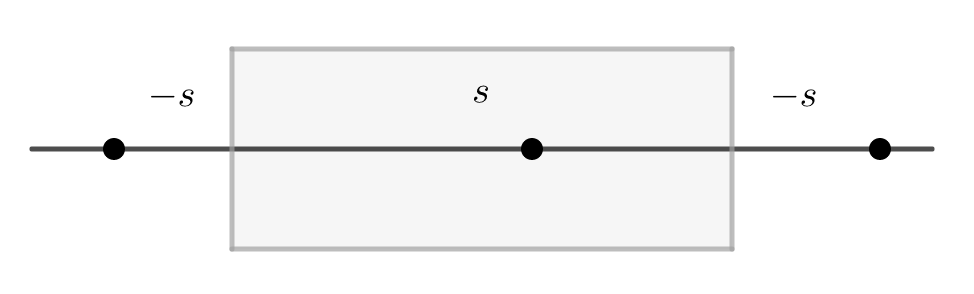
\includegraphics[width=0.9\textwidth]{Question33.png}
        \caption{}
    \end{subfigure}
     \begin{subfigure}[t]{0.4\textwidth}
        \centering
        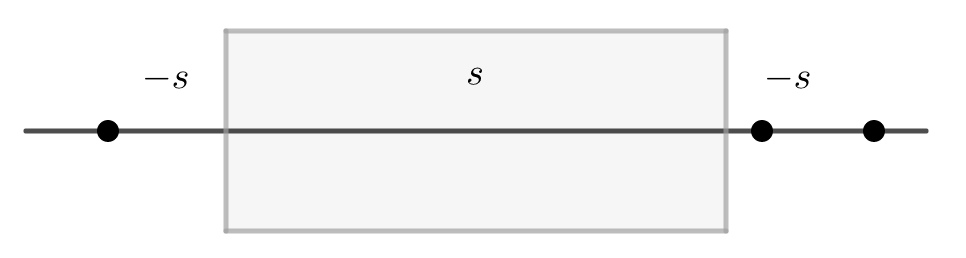
\includegraphics[width=0.9\textwidth]{Question34.png}
        \caption{}
    \end{subfigure}
    \caption{Proof that $\text{VCdim}(\mathcal{H}) \geq 3$.}
    \label{fig: question31}
\end{figure}

\item $\text{VCdim}(\mathcal{H}) \leq 3$: There does not exist a hypothesis $h \in \mathcal{H}$ that lables the situation on figure \ref{fig: question32}. From here we can conclude $\text{VCdim}(\mathcal{H}) \leq 3$.

\begin{figure}[h!]
    \centering
        
\includegraphics[width=0.9\textwidth]{Question35.png}
    \caption{Proof that $\text{VCdim}(\mathcal{H}) \leq 3$.}
    \label{fig: question32}
\end{figure}

\end{itemize}

\end{solution}
\end{question}


% 4th question
\begin{question}{\textbf{VC of union:} Let $\mathcal{H}_1,\dots, \mathcal{H}_r$ be hypothesis classes over some fixed domain set $\mathcal{X}$. Let $d = \max_i \text{VCdim}(\mathcal{H}_i)$ and assume for simplicity that $d \geq 3$.}
\begin{subquestion}{Prove that
\[
\text{VCdim}(\cup_{i = 1}^r \mathcal{H}_i) \leq 4d \log (2d) + 2 \log (r).
\]
}
\begin{solution}
First, denote a union class as $\mathcal{H}_{\cup} = \cup_{i = 1}^r \mathcal{H}_i$.
Second, assume that $\text{VCdim}(\mathcal{H}_{\cup}) = k$ and therefore $\mathcal{H}_{\cup}$ shatters a set of $k$ elements . Furthermore, the union class can produce all $2^k$ possible labelings on these elements. 

Let's recall Sauer's lemma: Let $\mathcal{H}$ be a hypothesis class with $\text{VCdim}(\mathcal{H}) \leq d < \infty$. Then for all $m$,
\[
\Pi_{\mathcal{H}}(m) \leq m^d
\]
From our assumption it follows:
\[
\Pi_{\mathcal{H}_{\cup}}(k) = 2^k
\]
The definition of shatter function gives as the following inequality:
\[
\Pi_{\mathcal{H}_{\cup}}(k) \leq \Pi_{\mathcal{H}_{1}}(k) + \cdots + \Pi_{\mathcal{H}_{r}}(k)
\]
Now, we can use Sauer's lemma on each summand:
\[
2^k = \Pi_{\mathcal{H}_{\cup}}(k) \leq \Pi_{\mathcal{H}_{1}}(k) + \cdots + \Pi_{\mathcal{H}_{r}}(k) \leq \underbrace{k^d + \cdots k^d}_r = rk^d
\]
If we use logarithm on the inequality, we get:
\begin{equation}
k \leq d\log k + \log r
\label{eq: quation41}
\end{equation}

In the next step we are going to use Lemma A.2 from the book, which says: Let $a \geq 1$ and $b > 0$. Then $x \geq 4a \log(2a) + 2b \implies x \geq a \log(x) + b$.

Let's assume that $\text{VCdim}(\mathcal{H}_{\cup}) > 4d \log (2d) + 2 \log (r)$. From our first assumption we get:
\[
k > 4d \log (2d) + 2 \log (r)
\]
Now, we can use Lemma A.2 (where $a = d \geq 3$, $b = \log r > 0$):
\[
k > d\log k + \log r
\]
We got into a contradiction with \eqref{eq: quation41}, this means that our assumption was not correct and it holds:
\[
\text{VCdim}(\mathcal{H}_{\cup}) \leq 4d \log (2d) + 2 \log (r)
\]
\end{solution}
\end{subquestion}

\begin{subquestion}{Prove that for $r = 2$ it holds that
\[
\text{VCdim}(\mathcal{H}_1 \cup \mathcal{H}_2 \leq 2d + 1)
\]
}
\begin{solution}
% https://cs.nyu.edu/~mohri/ml/ml10/sol2.pdf
\end{solution}
\end{subquestion}
\end{question}

\bibliographystyle{plain}
\bibliography{references}
\end{document}